\documentclass[11pt, a4paper]{article}

\usepackage[english]{babel}
\usepackage{sleek}
\usepackage{common}

\title{Introduction to Artificial Intelligence (INFO8006)}
\subtitle{Exercises 1 -- Solving problems by searching}
\date{\today}

\def\Astar{$\text{A}^*$}

\begin{document}

\maketitle

\section*{Learning outcomes}

At the end of this session you should be able to
\begin{itemize}[noitemsep]
    \item formulate search problems rigorously;
    \item analyze the algorithms to perform uninformed search (depth-first, breadth-first, uniform-cost) and informed search (greedy, \Astar{});
    \item apply these algorithms in fully observable and deterministic environments.
\end{itemize}

\section{Search algorithms}

\begin{figure}[h]
    \centering
    \scalebox{0.75}{\begin{tikzpicture}[node distance = 4cm]
        \node[state] (S) {S(tart)\\$h=11$};
        \node[state] (A) [above right of=S] {A\\$h=20$};
        \node[state] (B) [right of=S] {B\\$h=12$};
        \node[state] (C) [below right of=S] {C\\$h=10$};
        \node[state] (D) [below right of=B] {D\\$h=3$};
        \node[state] (E) [above right of=B] {E\\$h=19$};
        \node[state] (G) [right of=D] {G(oal)};

        \path[-] (S) edge node[fill=white] {1} (A);
        \path[-] (S) edge node[fill=white] {4} (B);
        \path[-] (S) edge node[fill=white] {3} (C);
        \path[-] (B) edge node[fill=white] {7} (D);
        \path[-] (B) edge node[fill=white] {5} (E);
        \path[-] (D) edge node[fill=white] {10} (G);
        \path[-] (E) edge node[fill=white] {1} (D);
        \path[-] (E) edge node[fill=white] {20} (G);
        \path[-] (C) edge node[fill=white] {2} (B);
        \path[-] (A) edge node[fill=white] {5} (B);
    \end{tikzpicture}}
\end{figure}

For each of the following search algorithms, apply the \textsc{Graph-Search} algorithm (lecture 2, slide 62) and give the order in which the states, represented by the nodes of this undirected graph, are expanded, as well as the final path returned by the algorithm. If two nodes are in competition to be expanded, the conflict is resolved by alphabetical order.

\begin{enumerate}
    \item Depth-First Search (DFS)

    \begin{solution}
        We use a Last-In First-Out (LIFO) fringe, \ie{} a \emph{stack}, to perform the search. In this stack, we keep track of the states that are reachable from the visited (closed) states. These states are annotated with the state they were expanded from, which allows to reconstruct the path at the end. At each step, the state at the \emph{top} of the stack is \emph{popped}. If it was not visited previously, it is expanded, which consists in \emph{pushing} its neighbors to the top of the stack.

        \begin{table}[H]
            \centering
            \begin{tabular}{l|l|c}
                \toprule
                Fringe (LIFO stack) & Closed & Expand \\
                \midrule
                S & & S \\
                C(S), B(S), A(S) & S & A(S) \\
                C(S), B(S), B(A) & S, A & B(A) \\
                C(S), E(B), D(B), C(B) & S, A, B & C(B) \\
                E(B), D(B) & S, A, B, C & D(B) \\
                E(B), G(D), E(D) & S, A, B, C, D & E(D) \\
                G(D), G(E) & S, A, B, C, D, E & G(E) \\
                \bottomrule
            \end{tabular}
        \end{table}

        For readability, we don't write the nodes currently in the fringe that are already in the closed set, since they will never be expanded.

        Expansion: S, A, B, C, D, E, G. Path: S, A, B, D, E, G.
    \end{solution}

    \item Breadth-First Search (BFS)

    \begin{solution}
        We use a First-In First-Out (FIFO) fringe, \ie{} a \emph{queue}, to keep track of the reachable states. At each step, the state at the \emph{front} of the queue is popped. If it was not visited previously, it is expanded, which consists in pushing its neighbors to the \emph{back} of the queue.

        \begin{table}[h]
            \centering
            \begin{tabular}{l|l|c}
                \toprule
                Fringe (FIFO queue) & Closed & Expand \\
                \midrule
                S & & S \\
                C(S), B(S), A(S) & S & A(S) \\
                B(A), C(S), B(S) & S, A & B(S) \\
                E(B), D(B), C(B), C(S) & S, A, B & C(S) \\
                E(B), D(B) & S, A, B, C & D(B) \\
                G(D), E(D), E(B) & S, A, B, C, D & E(B) \\
                G(E), G(D) & S, A, B, C, D, E & G(D) \\
                \bottomrule
            \end{tabular}
        \end{table}

        Expansion: S, A, B, C, D, E, G. Path: S, B, D, G.
    \end{solution}

    \item Uniform-Cost search (UCS)

    \begin{solution}
        The fringe is a \emph{priority} queue. The priority of a node $n$ in the queue is its cumulative cost $g(n)$.

        \begin{table}[h]
            \centering
            \begin{tabular}{l|l|c}
                \toprule
                Fringe (priority queue) & Closed & Expand \\
                \midrule
                S(0) & & S(0) \\
                B(S, 4), C(S, 3), A(S, 1) & S & A(S, 1) \\
                B(A, 6), B(S, 4), C(S, 3) & S, A & C(S, 3) \\
                B(A, 6), B(C, 5), B(S, 4) & S, A, C & B(S, 4) \\
                D(B, 11), E(B, 9) & S, A, C, B & E(B, 9) \\
                D(B, 11), D(E, 10) & S, A, C, B, E & D(E, 10) \\
                G(D, 20) & S, A, C, B, E, D & G(D, 20) \\
                \bottomrule
            \end{tabular}
        \end{table}

        Expansion: S, A, C, B, E, D, G. Path: S, B, E, D, G.
    \end{solution}

    \item Greedy search

    \begin{solution}
        The fringe is also a \emph{priority} queue, but the priority of a node $n$ in the queue is its \emph{heuristic} cost $h(n)$.

        \begin{table}[h]
            \centering
            \begin{tabular}{l|l|c}
                \toprule
                Fringe (priority queue) & Closed & Expand \\
                \midrule
                S(11) & & S(11) \\
                A(S, 20), B(S, 12), C(S, 10) & S & C(S, 10) \\
                A(S, 20), B(C, 12), B(S, 12) & S, C & B(S, 12) \\
                A(S, 20), E(B, 19), D(B, 3) & S, C, B & D(B, 3) \\
                A(S, 20), E(D, 19), E(B, 19), G(D, 0) & S, C, B, D & G(D, 0) \\
                \bottomrule
            \end{tabular}
        \end{table}

        Expansion: S, C, B, D, G. Path: S, B, D, G.
    \end{solution}

    \item \Astar{}

    \begin{solution}
    The priority of a node $n$ is the \emph{estimated} cost $f(n) = g(n) + h(n)$ of the cheapest solution through $n$.
    \end{solution}

    \begin{enumerate}
        \item Is the heuristic admissible ? If not, make it admissible.

        \begin{solution}
            A heuristic $h$ is admissible if $0 \leq h(n) \leq h^*(n)$, where $h^*(n)$ is the true forward cost of $n$. In the graph, $h(\text{E}) = 19$ is larger than $h^*(\text{E}) = 11$, making $h$ non-admissible. This is problematic as it means E (and G) would be expanded before D.

            Setting $h(\text{E}) = 11$ is sufficient to make $h$ admissible.
        \end{solution}

        \item Is the heuristic consistent ? If not, can we apply \textsc{Graph-Search} ?

        \begin{solution}
            In a graph, a heuristic $h$ is consistent if $h(n) \leq c(n, n') + h(n')$ for all node $n'$ reachable from $n$, where $c(n, n')$ is the step cost from $n$ to $n'$. Because this graph is undirected, unless $c(n, n') \geq \abs{h(n') - h(n)}$ for all pair of neighbors $(n, n')$ (which is not the case), it cannot be consistent.

            This is problematic as it could create situations where a node has been expanded within a path that is not optimal, and cannot be re-expanded later on within the optimal one. Hence, the algorithm loses its optimality.

            Fortunately, there is a modification of \textsc{Graph-Search} that can handle inconsistent heuristics. If we annotate the nodes in the closed set with the priority at which they were expanded, we obtain the capacity to re-expand a node if it has a better (lower) priority than before. The priority in the closed set is then updated.
        \end{solution}
    \end{enumerate}

    \begin{solution}
        We apply the modified algorithm with the admissible heuristic.

        \begin{table}[h]
            \centering
            \begin{tabular}{l|l|c}
                \toprule
                Fringe (priority queue) & Closed & Expand \\
                \midrule
                S(11) & & S(11) \\
                A(S, 21), B(S, 16), C(S, 13) & S(11) & C(S, 13) \\
                A(S, 21), B(C, 17), B(S, 16) & S(11), C(13) & B(S, 16) \\
                A(B, 29), A(S, 21), E(B, 20), D(B, 14) & S(11), C(13), B(16) & D(B, 14) \\
                A(B, 29), E(D, 23), G(D, 21), A(S, 21), E(B, 20) & S(11), C(13), B(16), D(14) & E(B, 20) \\
                A(B, 29), G(D, 21), A(S, 21), D(E, 13) & S(11), C(13), B(16), D(14), E(20) & D(E, 13) \\
                A(B, 29), G(D, 21), A(S, 21), G(D, 20) & S(11), C(13), B(16), D(13), E(20) & G(D, 20) \\
                \bottomrule
            \end{tabular}
        \end{table}

        Expansion: S, C, B, D, E, D, G. Path: S, B, E, D, G.
    \end{solution}
\end{enumerate}

\newpage

\section{Maze Car (UC Berkeley CS188, Spring 2014)}

\begin{figure}[h]
    \centering
    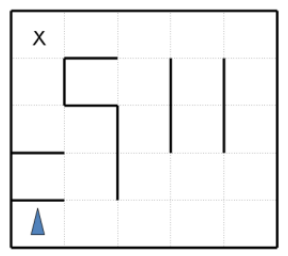
\includegraphics[width=0.3\linewidth]{figures/e1_maze.png}
\end{figure}

Consider a car agent which has to exit a maze. At all time-steps, the agent points at direction $d \in$ (N, S, E, W). With a single action, the agent can either move forward at an adjustable velocity $v \in [0, V]$ or turn. The turning actions are \texttt{left} and \texttt{right}, which change the agent's direction by 90 degrees. Turning is only permitted when the velocity is zero (and leaves it at zero). The moving actions are \texttt{faster} and \texttt{slower}. The action \texttt{faster} increments the velocity by 1 and \texttt{slower} decrements the velocity by 1; in both cases the agent then moves a number of squares equal to its \emph{new} velocity. Any action that would result in a collision with a wall is illegal. Any action that would reduce $v$ below 0 or above a maximum speed $V$ is also illegal. The agent's goal is to find a plan which parks it (stationary) on the exit square using as few actions (time steps) as possible.

As an example, in the hereabove maze, if the agent is initially stationary, it might first turn to the east using \texttt{right}, then move one square east using \texttt{faster}, then two more squares east using \texttt{faster} again. However, the agent will have to slow to take the turn.

\begin{enumerate}
    \item For a grid of size $M \times N$, what is the size of the state space? Assume that all configurations are reachable from the starting state.

    \begin{solution}
        $N \times M \times 4 \times (V + 1)$
    \end{solution}

    \item What is the maximum branching factor of this problem? Assume that illegal actions are simply not returned by the successor function.

    \begin{solution}
        The maximum branching factor is 3, and this happens when the agent is stationary. While stationary, it can take the following 3 actions: \texttt{faster}, \texttt{left}, \texttt{right}.
    \end{solution}

    \item Is the Manhattan distance from the agent's location to the exit's location admissible?

    \begin{solution}
        No because it does not take the velocity of the agent into account. For instance, in a long straight path, the number of steps could be smaller than the number of squares.
    \end{solution}

    \item If we used an inadmissible heuristic in \Astar{} tree search, could it change the completeness of the search? And the optimality ?

    \begin{solution}
        With an inadmissible heuristic, \Astar{} will still find a final state if there exists a reachable one (complete), but it could stop the search before finding the optimal one (non optimal).
    \end{solution}

    \item State and motivate a non-trivial admissible heuristic for this problem.

    \begin{solution}
        Some examples of admissible heuristics are:
        \begin{itemize}
            \item The Manhattan distance divided by the max speed $V$.
            \item We can improve the above heuristic by adding the current velocity $v$, as the agent has to slow down to 0 before reaching its goal. This heuristic \emph{dominates} the first one as it is always larger (or equal), but is still admissible as it never overestimates the true forward cost.
        \end{itemize}
    \end{solution}

    \item Give a general advantage that an inadmissible heuristic might have over an admissible one.

    \begin{solution}
        The time to solve an \Astar{} tree search problem is a function of two factors: the number of nodes expanded, and the time spent per node.
        \begin{itemize}
            \item An inadmissible heuristic may be faster to compute, leading to a solution that is obtained faster due to less time spent per node.
            \item Admissible heuristics are sometimes too conservative (well below $h^*$). An inadmissible heuristic could be a better estimate of the true forward cost $h^*$ (although it will overestimate at times), thus expanding less nodes.
        \end{itemize}
        We lose the guarantee of optimality by using an inadmissible heuristic. However, sometimes, we may be okay with finding a suboptimal solution faster.
    \end{solution}
\end{enumerate}

\newpage

\section{Heuristics (UC Berkeley CS188, Spring 2019)}

Consider a graph search problem where all edges have a unit cost and the optimal solution has cost $C^*$. Let $h(n)$ be a heuristic which is $\max \cbk{h^*(n) - k, 0}$, where $h^*(n)$ is the true forward cost of $n$ and $k \leq C^*$ is a non-negative constant.

\begin{enumerate}
    \item Is $h$ admissible?

    \begin{solution}
        Yes. If $h^* \geq k$, $h^* - k \leq h^*$, otherwise $0 \leq h^*$.
    \end{solution}

    \item Which of the following is the most reasonable description of how much more work will be done, \ie{} how many more nodes will be expanded, with heuristic $h$ compared to $h^*$, as a function of $k$?

    \begin{enumerate}
        \item Constant in $k$
        \item Linear in $k$
        \item Exponential in $k$
        \item Unbounded
    \end{enumerate}

    \begin{solution}
        With this heuristic, all nodes $n$ such that $h^*(n) \leq k$, \ie{} within distance $k$ from the objective, will have have a null heuristic. Assuming a node can have up to $p$ parents, there is at most $p^k$ such node and the algorithm will expand all of them, in the worst case. Thus, the additional work is exponential in $k$.
    \end{solution}
\end{enumerate}

\newpage

\section{Search algorithms}

\begin{figure}[h]
    \centering
    \scalebox{0.75}{\begin{tikzpicture}[node distance = 4cm]
        \node[state] (S) {S(tart)};
        \node[state] (A) [above right of=S] {A};
        \node[state] (B) [right of=A] {B};
        \node[state] (C) [below of=B] {C};
        \node[state] (D) [below right of=B] {D};
        \node[state] (G) [below of=D] {G(oal)};

        \path[-] (S) edge node[fill=white] {1} (A);
        \path[-] (S) edge node[fill=white] {12} (G);
        \path[-] (A) edge node[fill=white] {3} (B);
        \path[-] (A) edge node[fill=white] {1} (C);
        \path[-] (B) edge node[fill=white] {3} (D);
        \path[-] (C) edge node[fill=white] {1} (D);
        \path[-] (C) edge node[fill=white] {2} (G);
        \path[-] (D) edge node[fill=white] {3} (G);
    \end{tikzpicture}}
\end{figure}

For each of the following search algorithms, give the order in which states are expanded as well as the final path returned by the algorithm. If two nodes are in competition to be expanded, the conflict is resolved by alphabetical order.

\begin{enumerate}
    \item Depth-First search (DFS)

    \begin{solution}
        Expansion: S, A, B, D, C, G. Path: S, A, B, D, C, G.
    \end{solution}

    \item Breadth-First Search (BFS)

    \begin{solution}
        Expansion: S, A, G. Path: S, G.
    \end{solution}

    \item Uniform-Cost search (UCS)

    \begin{solution}
        Expansion: S, A, C, D, B, G. Path: S, A, C, G.
    \end{solution}

    \item Consider the following heuristics:
    \begin{table}[h]
        \centering
        \begin{tabular}{c|cc}
            \toprule
            State & $h_1$ & $h_2$ \\
            \midrule
            S & 5 & 4\\
            A & 3 & 2\\
            B & 6 & 6\\
            C & 2 & 1\\
            D & 3 & 3\\
            G & 0 & 0\\
            \bottomrule
        \end{tabular}
    \end{table}
    which one is not admissible? Why?

    \begin{solution}
        The heuristic $h_1$ is not admissible because the real cost from S to G is 4 which is smaller than 5.
    \end{solution}

    \item \Astar{} (with the admissible heuristic)

    \begin{solution}
        Expansion: S, A, C, G. Path: S, A, C, G.
    \end{solution}
\end{enumerate}

\newpage

\section{The hive (UC Berkeley CS188, Spring 2019)}

The hive of insects needs your help. You control an insect in a rectangular maze-like environment of size $M \times N$, as shown on the Figure below. At each time-step, the insect can move into a free adjacent cell or stay in its current location. All actions have a unit cost.

\begin{figure}[h]
    \centering
    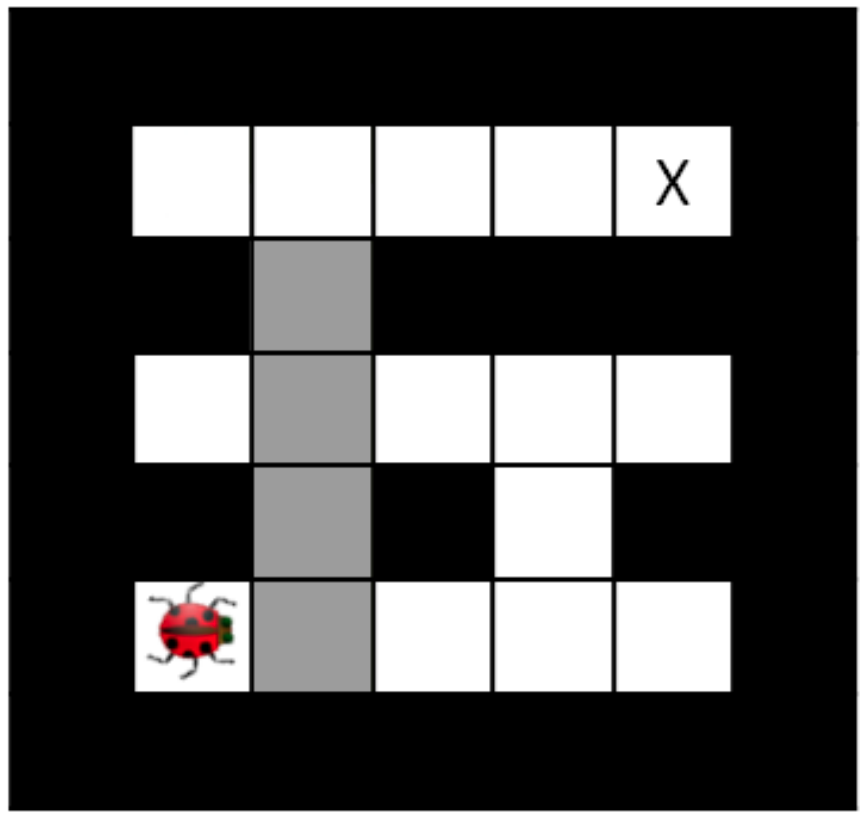
\includegraphics[width=0.3\linewidth]{figures/e1_hive.png}
\end{figure}

In this particular case, the insect must pass through a series of partially flooded tunnels, as illustrated by the gray cells on the map. The insect can hold its breath for $A$ time-steps in a row. Moving into a flooded cell requires your insect to consume 1 unit of air, while moving into a free cell refills its air supply.

\begin{itemize}
    \item Give a minimal state space for this problem (do not include extra information). You should answer for a general instance of the problem, not the specific map above.

    \begin{solution}
        The position of the insect  as well as the number of unit of air it has left. $s = (x, y, u_a) \in [1, M] \times [1, N] \times [1, A]$.
    \end{solution}

    \item Give the size of your state space.

    \begin{solution}
        $M\times N \times A$
    \end{solution}
\end{itemize}

\newpage

\section*{Supplementary materials}

\begin{itemize}
    \item Search (UC Berkeley CS188, Spring 2014 Section 0).

    \qrcode{http://ai.berkeley.edu/sections/section_0_v55LOfoUUwiW1k6Nchnk3Dw6WQuTW8.pdf}

    \item Search (UC Berkeley CS188, Spring 2014 Section 1).

    \qrcode{http://ai.berkeley.edu/sections/section_1_0hzy6TFupb1Z3bckfRXdC5KYpsdZOE.pdf}

    \item Chapter 3 of the reference textbook.
\end{itemize}

\end{document}
